% CONTEXTE : 
% Une Ecole primaire se dote de moyens informatiques de manière à pouvoir automatiser sa gestion.
% • Un élève est caractérisé par les informations suivantes : NumEleve, NomElève, PrénomElève,
% AdresseElève, Date Naissance, sexe ; il est inscrit dans une classe pour une année donnée.
% • On souhaite aussi conserver des données concernant les parents de l’enfant (à définir)
% • Un professeur est caractérisé par les informations suivantes : NomProfesseur, PrénomProfesseur,
% AdresseProfesseur, Departement, DateEntrée, Numéro de téléphone, Age.
% • Une classe est caractérisée par son numéro et son libellé (Cours Préparatoire_1, Cours
% Préparatoire_2, Cours Elémentaire1_1,….)
% • Chaque classe, pour une année donnée est associée à un seul professeur.
% • Chaque matière est caractérisée par un code et un libellé. Dans une même matière, mais à des
% dates différentes, un élève peut avoir plusieurs notes.
% • Certains professeurs sont dispensés d’enseignement (ex : directeurs)

\documentclass[a4paper,12pt]{article}
\usepackage[utf8]{inputenc}
\usepackage[T1]{fontenc}
\usepackage[french]{babel}
\usepackage{graphicx}
\usepackage{amsmath}
\usepackage{amssymb}
\usepackage{hyperref}
\usepackage{geometry}
\usepackage{float}
\usepackage{fancyhdr}
\geometry{hmargin=2.5cm, vmargin=3cm}


\pagestyle{fancy}
\fancyhf{}
\rhead{SANNA Thomas, L3STI}
\lhead{Projet Ecole - Bases de Données}
\rfoot{Page \thepage}

\title{Rapport de TP \\ Projet Ecole - Bases de Données}
\author{Thomas SANNA}
\date{\today}

\begin{document}

\maketitle

\tableofcontents

\break
\section{Partie Analyse / Conception}
\subsection{Dictionnaire de données}
\begin{itemize}
  \item NumEleve (INT)
  \item NomEleve (chaine de caracteres)
  \item PrenomEleve (chaine de caracteres)
  \item AdresseEleve (chaine de caracteres)
  \item DateNaissance (DATE)
  \item Sexe (CHAR)
  \item NumParent (INT)
  \item NomParent (chaine de caracteres)
  \item PrenomParent (chaine de caracteres)
  \item AdresseParent (chaine de caracteres)
  \item NumProfesseur (INT)
  \item NomProfesseur (chaine de caracteres)
  \item PrenomProfesseur (chaine de caracteres)
  \item AdresseProfesseur (chaine de caracteres)
  \item Departement (chaine de caracteres)
  \item DateEntree (DATE)
  \item NumTelephone (chaine de caracteres)
  \item Age (INT)
  \item NumClasse (INT)
  \item LibelleClasse (chaine de caracteres)
  \item AnneeScolaire (DATE)
  \item CodeMatiere (chaine de caracteres)
  \item LibelleMatiere (chaine de caracteres)
  \item DateNote (DATE)
  \item Note (DECIMAL)
\end{itemize}

\subsection{Couverture minimale}

\begin{figure}[H]
  \centering
  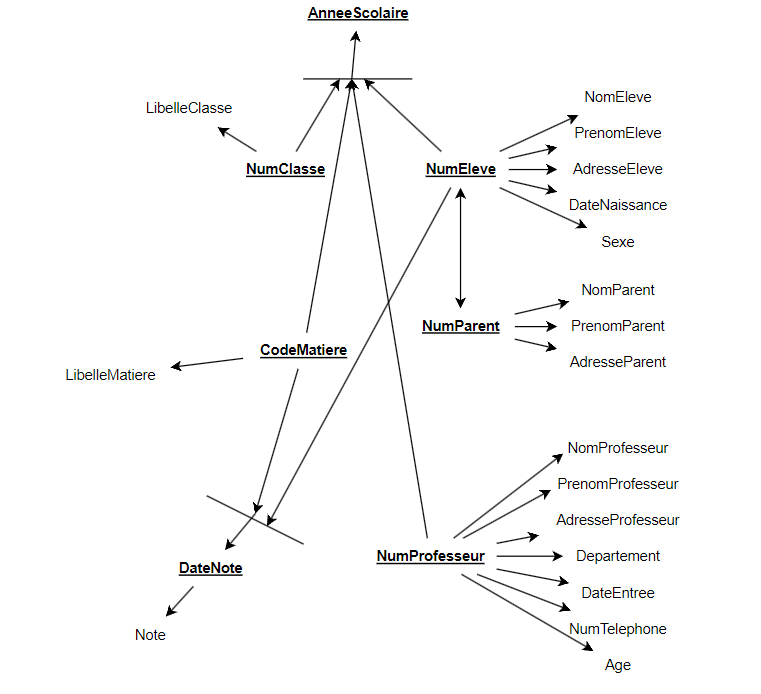
\includegraphics[width=0.8\textwidth]{img/couv.png}
  \caption{Couverture minimale}
\end{figure}

\subsection{MCD}

\begin{figure}[H]
  \centering
  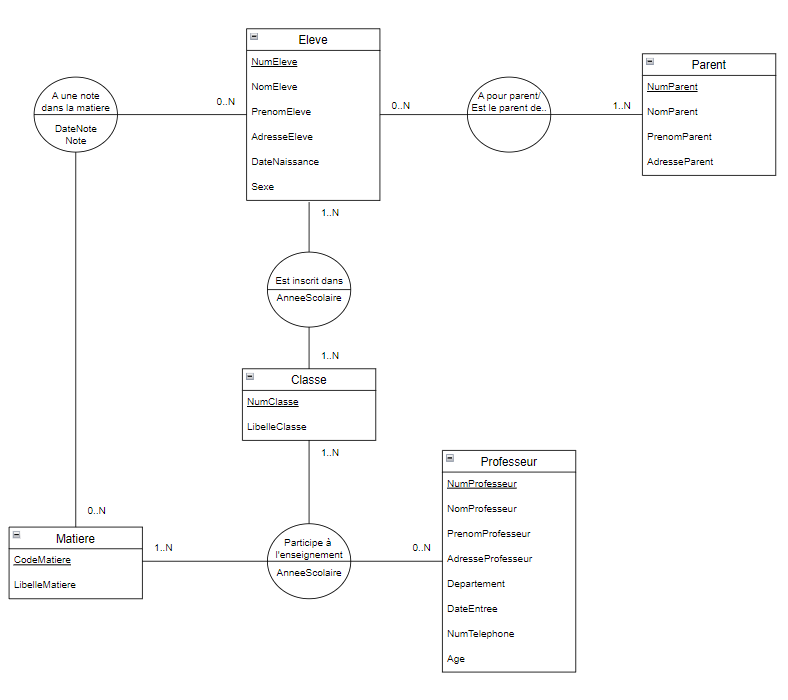
\includegraphics[width=0.8\textwidth]{img/mcd.png}
  \caption{Modèle Conceptuel de Données}
\end{figure}

\subsection{Schémas relationnel}
\begin{itemize}
  \item \textbf{Eleve} (\underline{NumEleve}, NomEleve, PrenomEleve, AdresseEleve, DateNaissance, Sexe)
  \item \textbf{Parent} (\underline{NumParent}, NomParent, PrenomParent, AdresseParent)
  \item \textbf{ParentEleve} (\underline{\#{NumParent}, \#{NumEleve}})
  \item \textbf{Professeur} (\underline{NumProfesseur}, NomProfesseur, PrenomProfesseur, AdresseProfesseur, Departement, DateEntree, NumTelephone, Age)
  \item \textbf{Classe} (\underline{NumClasse}, LibelleClasse)
  \item \textbf{Inscription} (\underline{AnneeScolaire, \#{NumEleve}}, \#{NumClasse})
  \item \textbf{Matiere} (\underline{CodeMatiere}, LibelleMatiere)
  \item \textbf{Enseignement} (\underline{\#{NumProfesseur}, \#{NumClasse}, \#{CodeMatiere}, AnneeScolaire})
  \item \textbf{Note} (\underline{NumEleve, \#{CodeMatiere}, DateNote}, Note)
\end{itemize}

\section{Algèbre Relationnelle}
\begin{itemize}
  \item \textbf{Requête 1} : Trouver tous les élèves de la classe nommée "ClasseX"
  \begin{align*}
      R1 &= \sigma_{LibelleClasse = 'ClasseX'}(Inscription) \\
      R2 &= (R1)_{NumEleve} \bowtie_{NumEleve} Eleve \\
      R3 &= \pi_{NomEleve, PrenomEleve}(R2)
  \end{align*}
  
  \item \textbf{Requête 2} : Trouver les notes de l'élève n°2 pour une la matière "MATH"
  \begin{align*}
      R1 &= \sigma_{NumEleve = 2}(Note) \\
      R2 &= \sigma_{CodeMatiere = 'MATH'}(R1) \\
      R3 &= \pi_{DateNote, Note}(R2)
  \end{align*}
  
  \item \textbf{Requête 3} : Trouver les professeurs d'un département donné
  \begin{align*}
      R1 &= \sigma_{Departement = 'D'}(Professeur) \\
      R2 &= \pi_{NomProfesseur, PrenomProfesseur}(R1)
  \end{align*}

  \item \textbf{Requête 4} : Liste des élèves et leurs parents pour une classe donnée
  \begin{align*}
      R1 &= \sigma_{NumClasse = 'X'}(Inscription) \\
      R2 &= (R1)_{NumEleve} \bowtie_{NumEleve} Eleve \\
      R3 &= (R2)_{NumEleve} \bowtie_{NumEleve} ParentEleve \\
      R4 &= (R3)_{NumParent} \bowtie_{NumParent} Parent \\
      R5 &= \pi_{NomEleve, PrenomEleve, NomParent, PrenomParent}(R4)
  \end{align*}

  \item \textbf{Requête 5} : Moyenne des notes par matière et par classe
  \begin{align*}
      R1 &= Note_{CodeMatiere} \bowtie_{CodeMatiere} Enseignement \\
      R2 &= \gamma_{NumClasse, CodeMatiere; AVG(Note) \rightarrow MoyenneNote}(R1) \\
      R3 &= (R2)_{CodeMatiere} \bowtie_{CodeMatiere} Matiere \\
      R4 &= \pi_{NumClasse, LibelleMatiere, MoyenneNote}(R3)
  \end{align*}

  \item \textbf{Requête 6} : Professeurs qui enseignent toutes les matières
  \begin{align*}
      R1 &= \pi_{CodeMatiere}(Matiere) \\
      R2 &= \pi_{NumProfesseur, CodeMatiere}(Enseignement) \\
      R3 &= (R2 \div R1)_{NumProfesseur} \bowtie_{NumProfesseur} Professeur \\
      R4 &= \pi_{NomProfesseur, PrenomProfesseur}(R3)
  \end{align*}

  \item \textbf{Requête 7} : Élèves ayant une moyenne supérieure à 15 dans toutes les matières
  \begin{align*}
      R1 &= \gamma_{NumEleve, CodeMatiere; AVG(Note) \rightarrow MoyenneNote}(Note) \\
      R2 &= \sigma_{MoyenneNote > 15}(R1) \\
      R3 &= \pi_{NumEleve}(R2) \div \pi_{CodeMatiere}(Matiere) \\
      R4 &= (R3)_{NumEleve} \bowtie_{NumEleve} Eleve \\
      R5 &= \pi_{NomEleve, PrenomEleve}(R4)
  \end{align*}

  \item \textbf{Requête 8} : Classes sans note inférieure à 10 ce semestre
  \begin{align*}
      R1 &= \sigma_{Note < 10}(Note) \\
      R2 &= (R1)_{NumEleve} \bowtie_{NumEleve} Inscription \\
      R3 &= \pi_{NumClasse}(Classe) - \pi_{NumClasse}(R2) \\
      R4 &= (R3)_{NumClasse} \bowtie_{NumClasse} Classe \\
      R5 &= \pi_{NumClasse, LibelleClasse}(R4)
  \end{align*}
\end{itemize}

\section{Partie Réalisation}

\subsection{Création des tables MYSQL}
\begin{verbatim}
-- Nom BDD : ecole_bdd

CREATE TABLE Eleve (
    NumEleve INT PRIMARY KEY,
    NomEleve VARCHAR(50) NOT NULL,
    PrenomEleve VARCHAR(50) NOT NULL,
    AdresseEleve VARCHAR(100),
    DateNaissance DATE,
    Sexe CHAR(1)
);

CREATE TABLE Parent (
    NumParent INT PRIMARY KEY,
    NomParent VARCHAR(50) NOT NULL,
    PrenomParent VARCHAR(50) NOT NULL,
    AdresseParent VARCHAR(100)
);

CREATE TABLE ParentEleve (
    NumParent INT,
    NumEleve INT,
    PRIMARY KEY (NumParent, NumEleve),
    FOREIGN KEY (NumParent) REFERENCES Parent(NumParent),
    FOREIGN KEY (NumEleve) REFERENCES Eleve(NumEleve)
);

CREATE TABLE Professeur (
    NumProfesseur INT PRIMARY KEY,
    NomProfesseur VARCHAR(50) NOT NULL,
    PrenomProfesseur VARCHAR(50) NOT NULL,
    AdresseProfesseur VARCHAR(100),
    Departement VARCHAR(50),
    DateEntree DATE,
    NumTelephone VARCHAR(15),
    Age INT
);

CREATE TABLE Classe (
    NumClasse INT PRIMARY KEY,
    LibelleClasse VARCHAR(50) NOT NULL
);

CREATE TABLE Inscription (
    AnneeScolaire YEAR,
    NumEleve INT,
    NumClasse INT,
    PRIMARY KEY (AnneeScolaire, NumEleve),
    FOREIGN KEY (NumEleve) REFERENCES Eleve(NumEleve),
    FOREIGN KEY (NumClasse) REFERENCES Classe(NumClasse)
);

CREATE TABLE Matiere (
    CodeMatiere VARCHAR(10) PRIMARY KEY,
    LibelleMatiere VARCHAR(50) NOT NULL
);

CREATE TABLE Enseignement (
    NumProfesseur INT,
    NumClasse INT,
    CodeMatiere VARCHAR(10),
    AnneeScolaire YEAR,
    PRIMARY KEY (NumProfesseur, NumClasse, CodeMatiere, AnneeScolaire),
    FOREIGN KEY (NumProfesseur) REFERENCES Professeur(NumProfesseur),
    FOREIGN KEY (NumClasse) REFERENCES Classe(NumClasse),
    FOREIGN KEY (CodeMatiere) REFERENCES Matiere(CodeMatiere)
);

CREATE TABLE Note (
    NumEleve INT,
    CodeMatiere VARCHAR(10),
    DateNote DATE,
    Note DECIMAL(4,2),
    PRIMARY KEY (NumEleve, CodeMatiere, DateNote),
    FOREIGN KEY (NumEleve) REFERENCES Eleve(NumEleve),
    FOREIGN KEY (CodeMatiere) REFERENCES Matiere(CodeMatiere),
    CHECK (Note >= 0 AND Note <= 20)
);
\end{verbatim}

\subsection{Site Web en PHP permettant de gérer les données}

\begin{figure}[H]
    \centering
    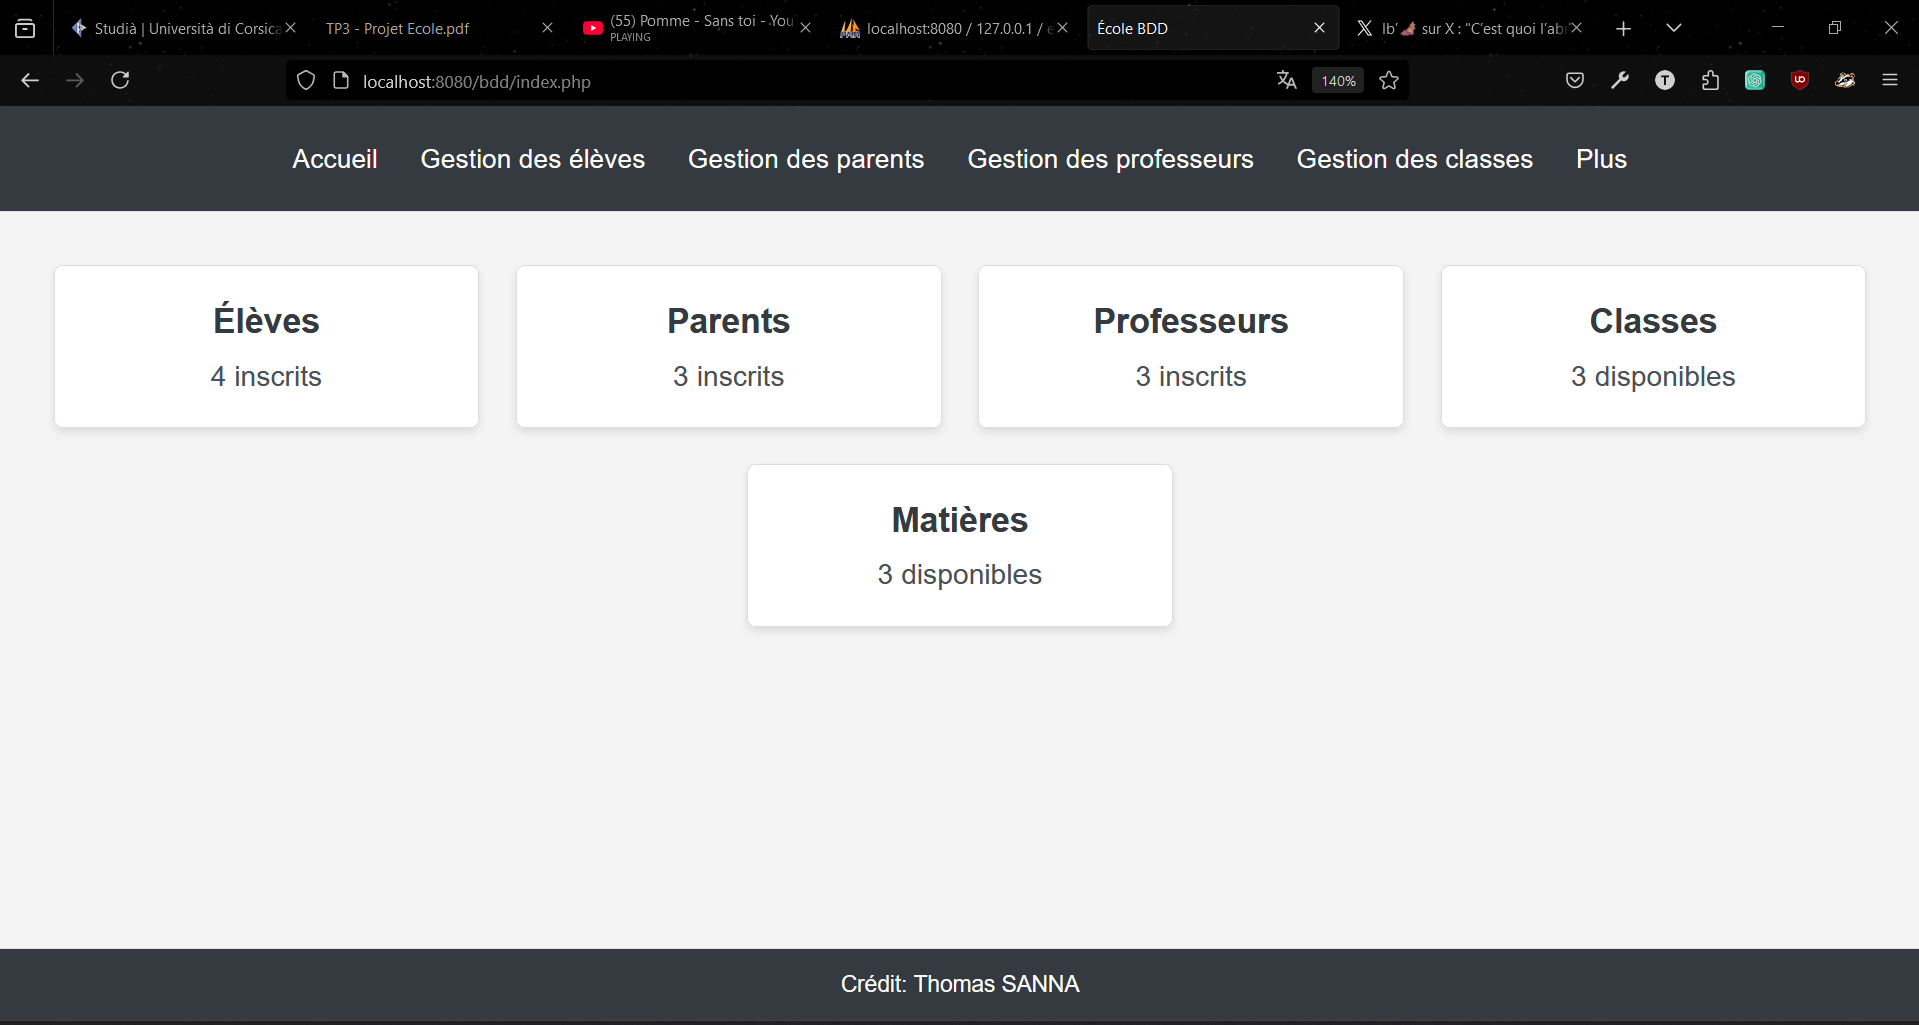
\includegraphics[width=0.8\textwidth]{imgSite/accueil.png}
    \caption{Page d'accueil}
\end{figure}

La page d'accueil permet de naviguer entre les différentes fonctionnalités du site.

\begin{figure}[H]
    \centering
    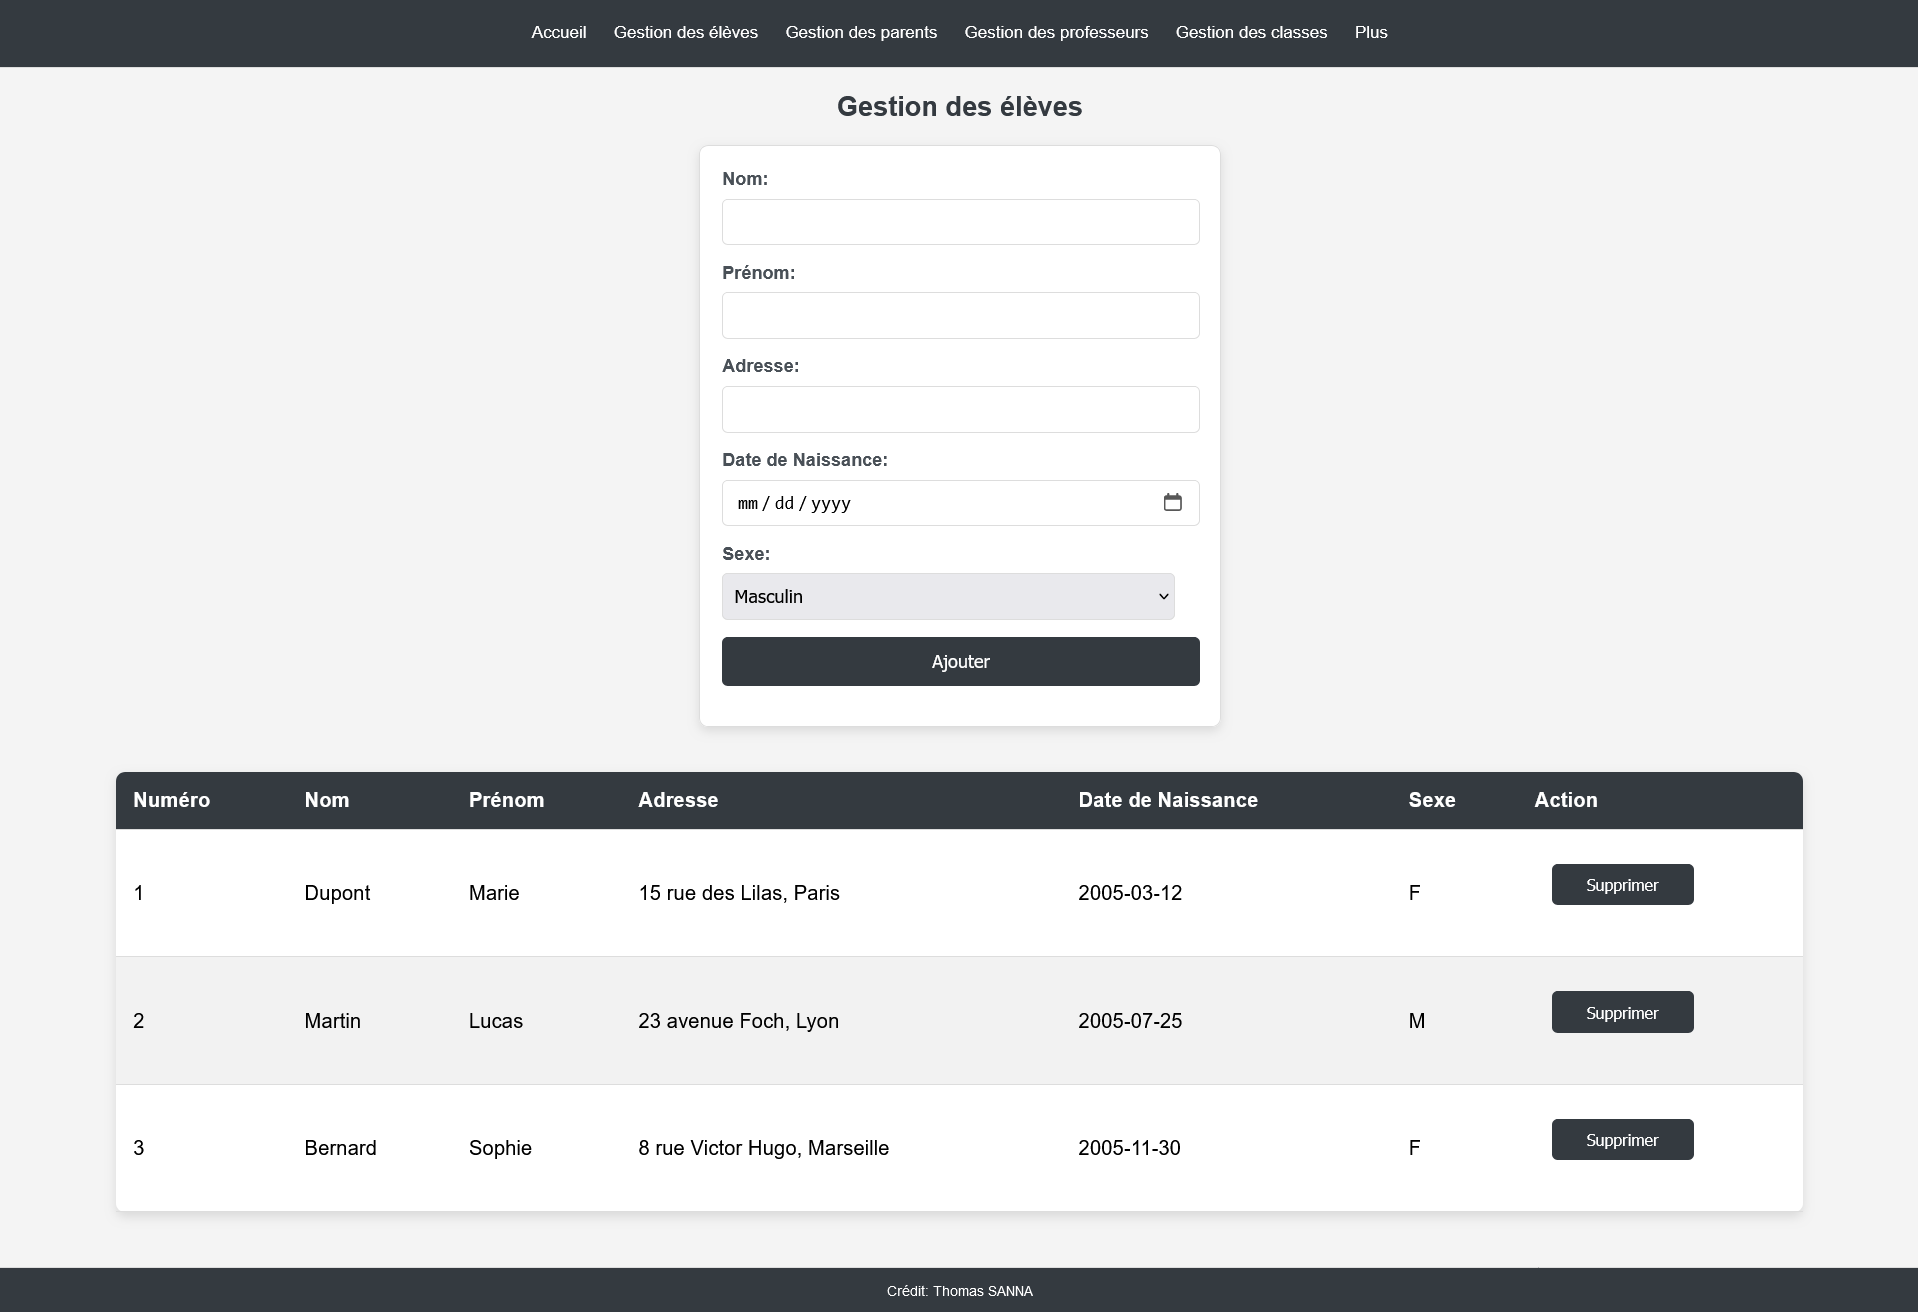
\includegraphics[width=0.8\textwidth]{imgSite/eleve.png}
    \caption{Liste des élèves}
\end{figure}

Cette page permet de visualiser la liste des élèves, d'en ajouter des nouveaux ou de les supprimer.

De la même manière, on peut visualiser les parents, les professeurs, les classes, les matières, les inscriptions et les notes.

\begin{figure}[H]
    \centering
    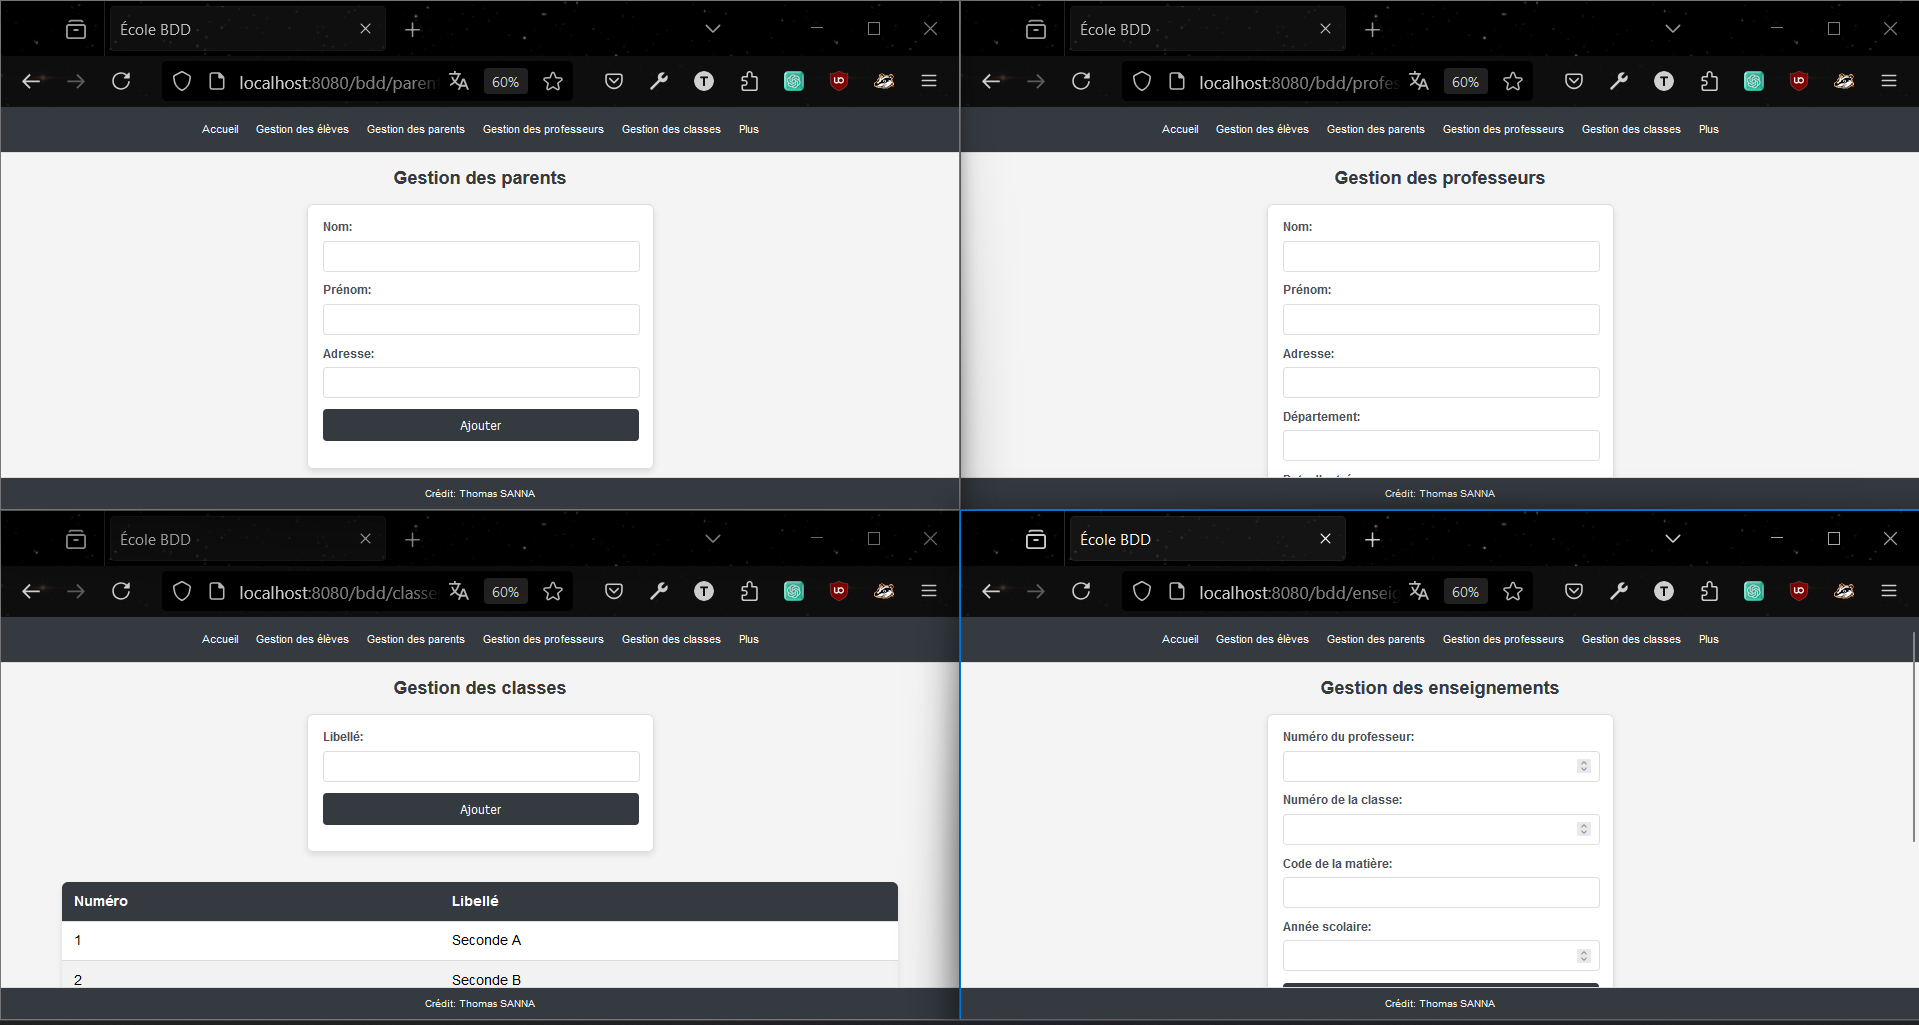
\includegraphics[width=0.8\textwidth]{imgSite/all.png}
    \caption{Autres pages permettant de gérer les données de l'école}
\end{figure}

\subsection{Autres fonctionnalités}

\begin{figure}[H]
    \centering
    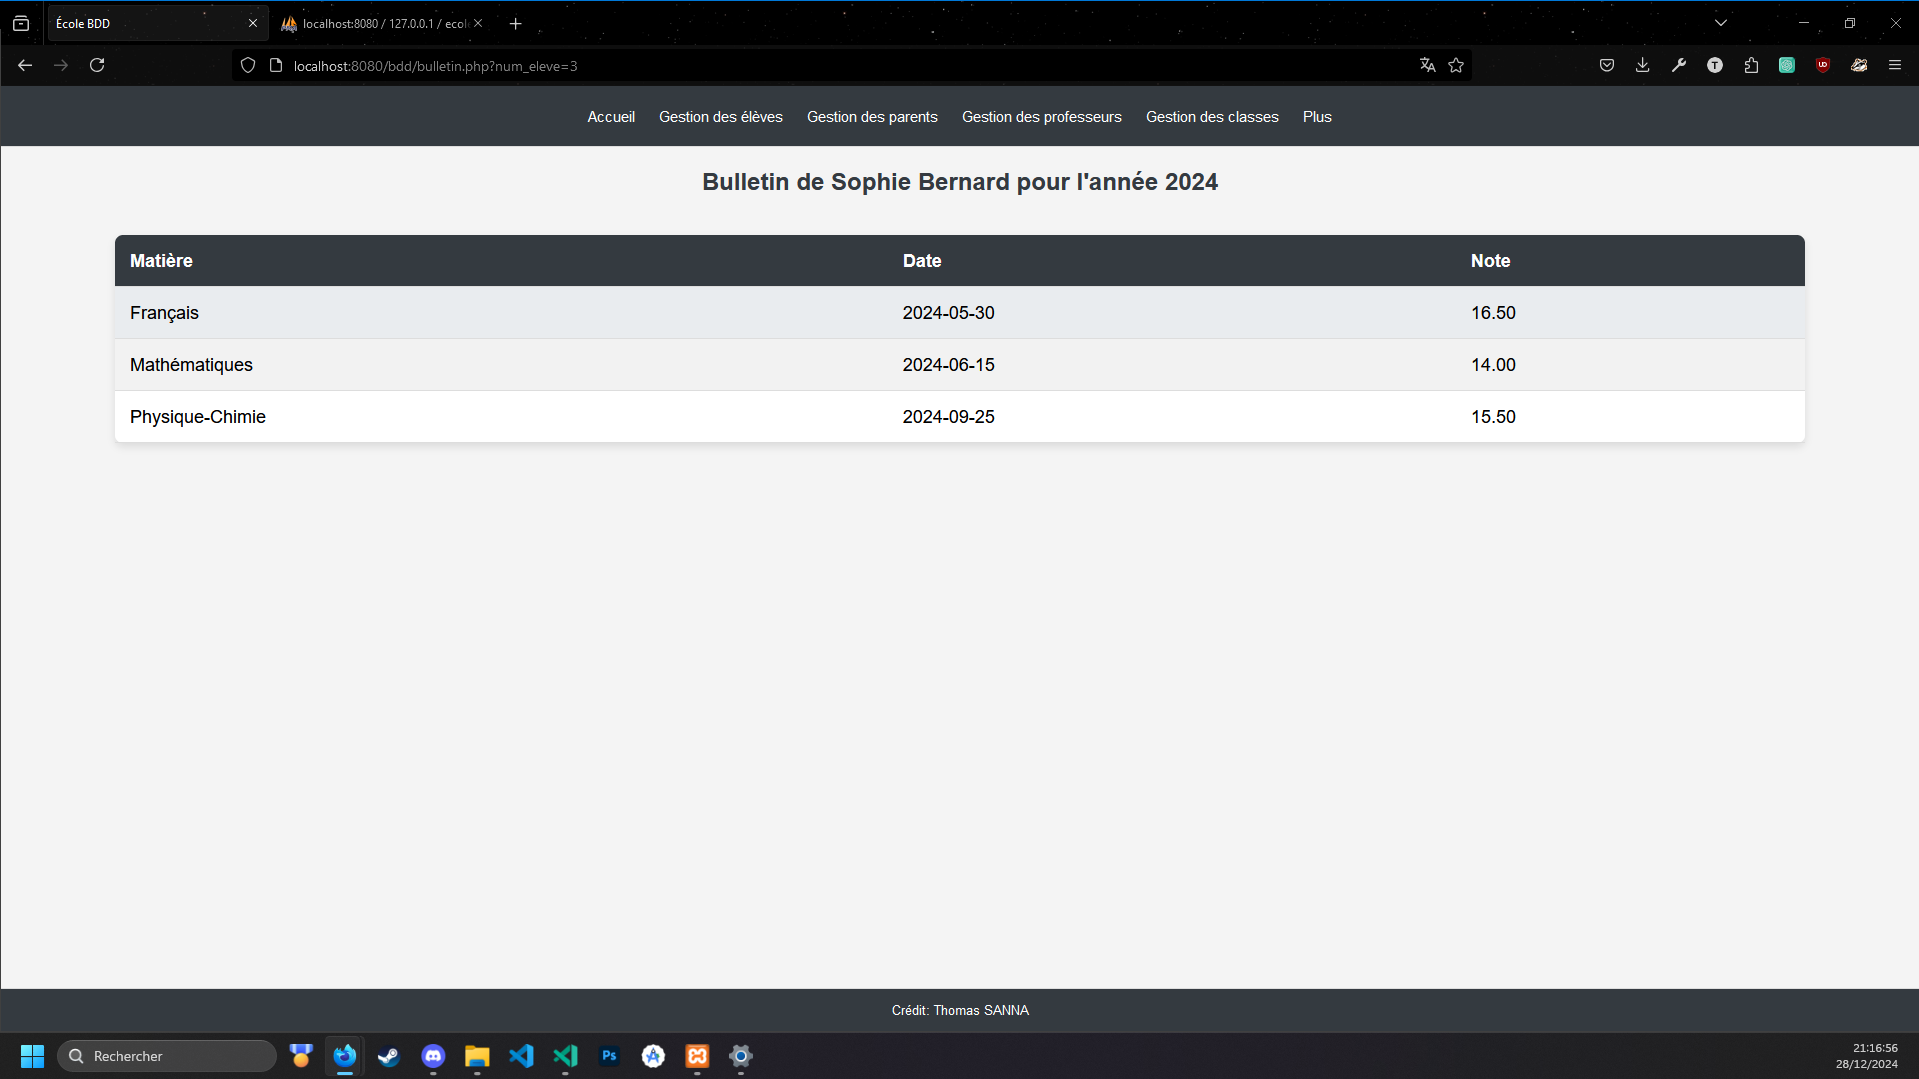
\includegraphics[width=0.8\textwidth]{imgSite/bulletin.png}
    \caption{Bulletin d'un élève choisit}
\end{figure}

Cette page permet de visualiser le bulletin d'un élève en particulier. On y retrouve les notes de l'élève pour chaque matière à une année donnée. 

\end{document}